% 09_tikz_graphics.tex
% TikZ diagrams and graphics for Siggraph and Digital Humanities
% Overleaf compatible: YES (TikZ + PGFPlots)

\documentclass[12pt,a4paper]{article}
\usepackage[utf8]{inputenc}
\usepackage[T1]{fontenc}
\usepackage{lmodern}
\usepackage[english]{babel}
\usepackage{hyperref}
\usepackage{cleveref}
\usepackage{tikz}
\usepackage{pgfplots}
\usepackage{pgfplotstable}
\usetikzlibrary{
    arrows.meta,
    positioning,
    shapes.geometric,
    shapes.misc,
    calc,
    decorations.pathreplacing,
    decorations.markings,
    matrix,
    fit,
    backgrounds,
    shadows,
    spy,
    external
}
\usepackage{float}

\pgfplotsset{compat=1.18}

\hypersetup{
    colorlinks=true,
    linkcolor=blue,
    citecolor=red,
    urlcolor=cyan
}

\title{TikZ Diagrams and Graphics for Siggraph \& Digital Humanities}
\author{Author Name}
\date{\today}

\begin{document}

\maketitle

\begin{abstract}
This example demonstrates TikZ/PGFPlots for creating publication-quality
diagrams: rendering pipelines, neural network architectures, stemma codicum,
parallel text alignment, coordinate systems, and data plots.
All graphics are vector-based and generated directly in \LaTeX.
\end{abstract}

% ============================================================
% 1. Rendering Pipeline (Siggraph)
% ============================================================
\section{Rendering Pipeline Diagram}
\label{sec:pipeline}

\begin{figure}[htbp]
\centering
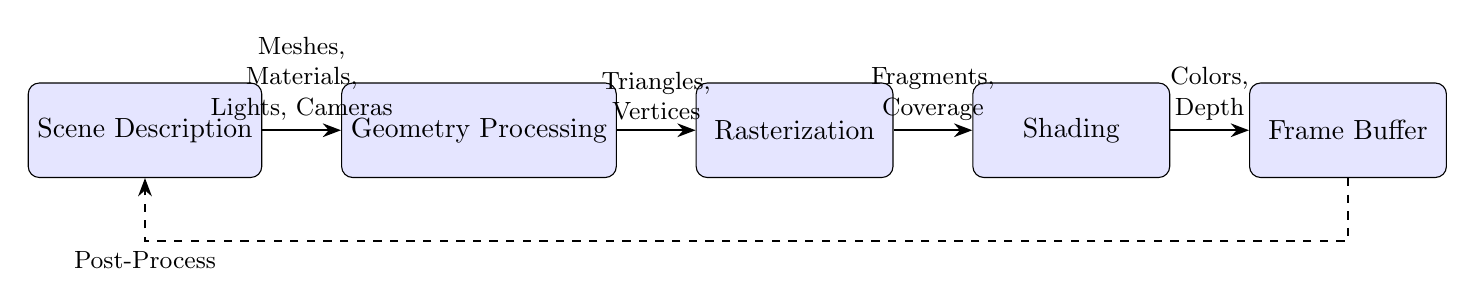
\begin{tikzpicture}[
    node distance=1.5cm and 1cm,
    box/.style={rectangle, draw, rounded corners, minimum height=1.2cm, minimum width=2.5cm, fill=blue!10},
    arrow/.style={-Stealth, thick},
    label/.style={font=\small, text width=2.5cm, align=center}
]
\node[box] (scene) {Scene Description};
\node[box, right=of scene] (geometry) {Geometry Processing};
\node[box, right=of geometry] (raster) {Rasterization};
\node[box, right=of raster] (shading) {Shading};
\node[box, right=of shading] (output) {Frame Buffer};

\draw[arrow] (scene) -- node[above, label] {Meshes, Materials,\\ Lights, Cameras} (geometry);
\draw[arrow] (geometry) -- node[above, label] {Triangles,\\ Vertices} (raster);
\draw[arrow] (raster) -- node[above, label] {Fragments,\\ Coverage} (shading);
\draw[arrow] (shading) -- node[above, label] {Colors,\\ Depth} (output);

% Feedback loop
\draw[arrow, dashed] (output.south) -- ++(0,-0.8) -| node[below, label, pos=0.5] {Post-Process} (scene.south);
\end{tikzpicture}
\caption{Real-time rendering pipeline}\label{fig:pipeline}
\end{figure}

% ============================================================
% 2. Ray Tracing Pipeline
% ============================================================
\section{Ray Tracing Pipeline}
\label{sec:raytrace}

\begin{figure}[htbp]
\centering
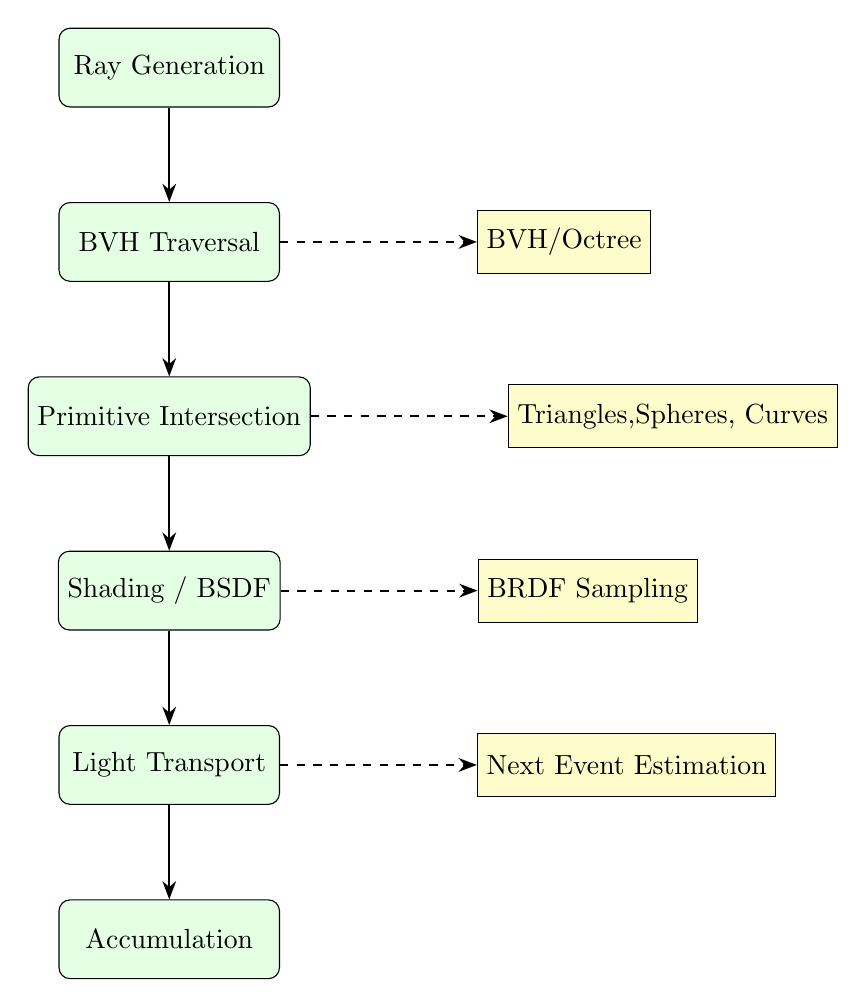
\begin{tikzpicture}[
    node distance=1.2cm and 1cm,
    stage/.style={rectangle, draw, rounded corners, minimum height=1cm, minimum width=2.8cm, fill=green!10},
    proc/.style={rectangle, draw, minimum height=0.8cm, minimum width=2.2cm, fill=yellow!20},
    arrow/.style={-Stealth, thick},
]
\node[stage] (gen) {Ray Generation};
\node[stage, below=of gen] (traverse) {BVH Traversal};
\node[stage, below=of traverse] (intersect) {Primitive Intersection};
\node[stage, below=of intersect] (shade) {Shading / BSDF};
\node[stage, below=of shade] (light) {Light Transport};
\node[stage, below=of light] (accum) {Accumulation};

\draw[arrow] (gen) -- (traverse);
\draw[arrow] (traverse) -- (intersect);
\draw[arrow] (intersect) -- (shade);
\draw[arrow] (shade) -- (light);
\draw[arrow] (light) -- (accum);

% Side notes
\node[proc, right=of traverse, xshift=1.5cm] (bvh) {BVH/Octree};
\node[proc, right=of intersect, xshift=1.5cm] (prim) {Triangles,\\ Spheres, Curves};
\node[proc, right=of shade, xshift=1.5cm] (bsdf) {BRDF Sampling};
\node[proc, right=of light, xshift=1.5cm] (li) {Next Event Estimation};

\draw[arrow, dashed] (traverse) -- (bvh);
\draw[arrow, dashed] (intersect) -- (prim);
\draw[arrow, dashed] (shade) -- (bsdf);
\draw[arrow, dashed] (light) -- (li);
\end{tikzpicture}
\caption{Path tracing pipeline with acceleration structures}\label{fig:raytrace}
\end{figure}

% ============================================================
% 3. Neural Network Architecture
% ============================================================
\section{Neural Network Architecture (NeRF/MLP)}
\label{sec:nnarch}

\begin{figure}[htbp]
\centering
\begin{tikzpicture}[
    layer/.style={rectangle, draw, minimum width=1.5cm, minimum height=3cm, fill=blue!5},
    neuron/.style={circle, draw, minimum size=6pt, inner sep=0, fill=blue!20},
    conn/.style={-Stealth, very thin, opacity=0.3},
    label/.style={font=\small, rotate=90, anchor=south}
]
% Input
\node[layer, label=below:Input $\gamma(\vb{x}), \gamma(\vb{d})$] (in) at (0,0) {};
\foreach \y in {-1.2,-0.6,0,0.6,1.2} {
    \node[neuron] at (0,\y) {};
}

% Hidden layers
\foreach \i/\x/\h/\lbl in {1/2.5/3.5/FC 256, 2/5/3.5/FC 256, 3/7.5/3.5/FC 256, 4/10/3.5/FC 256} {
    \node[layer, minimum height=\h cm, label=below:\lbl] (h\i) at (\x,0) {};
    \foreach \y in {-1.5,-0.9,-0.3,0.3,0.9,1.5} {
        \ifnum\i<4
            \node[neuron] at (\x,\y) {};
        \fi
    }
    % Skip connection at layer 4
    \ifnum\i=4
        \node[neuron, fill=red!20] at (\x,-1.5) {};
        \node[neuron, fill=red!20] at (\x,1.5) {};
    \fi
}

% Density output
\node[layer, minimum width=1.5cm, minimum height=1cm, label=below:$\sigma$] (dens) at (12.5,-1) {};
\node[neuron] at (12.5,-1) {};

% RGB output
\node[layer, minimum width=1.5cm, minimum height=1.5cm, label=below:RGB] (rgb) at (12.5,1) {};
\foreach \y in {0.5,1,1.5} {
    \node[neuron] at (12.5,\y) {};
}

% Connections
\foreach \i in {1,2,3,4} {
    \pgfmathtruncatemacro{\prev}{\i-1}
    \ifnum\prev=0
        \foreach \a in {-1.2,-0.6,0,0.6,1.2} {
            \foreach \b in {-1.5,-0.9,-0.3,0.3,0.9,1.5} {
                \draw[conn] (0,\a) -- (2.5,\b);
            }
        }
    \else
        \foreach \a in {-1.5,-0.9,-0.3,0.3,0.9,1.5} {
            \foreach \b in {-1.5,-0.9,-0.3,0.3,0.9,1.5} {
                \draw[conn] (\prev*2.5,\a) -- (\i*2.5,\b);
            }
        }
    \fi
}

% Skip connection
\draw[conn, red, thick] (0,-1.2) -- (10,-1.5);
\draw[conn, red, thick] (0,1.2) -- (10,1.5);

% Output connections
\foreach \a in {-1.5,-0.9,-0.3,0.3,0.9,1.5} {
    \draw[conn] (10,\a) -- (12.5,-1);
    \draw[conn] (10,\a) -- (12.5,1);
}
\end{tikzpicture}
\caption{NeRF MLP architecture with positional encoding and skip connections}\label{fig:nerf}
\end{figure}

% ============================================================
% 4. Stemma Codicum (Digital Humanities)
% ============================================================
\section{Stemma Codicum (Manuscript Genealogy)}
\label{sec:stemma}

\begin{figure}[htbp]
\centering
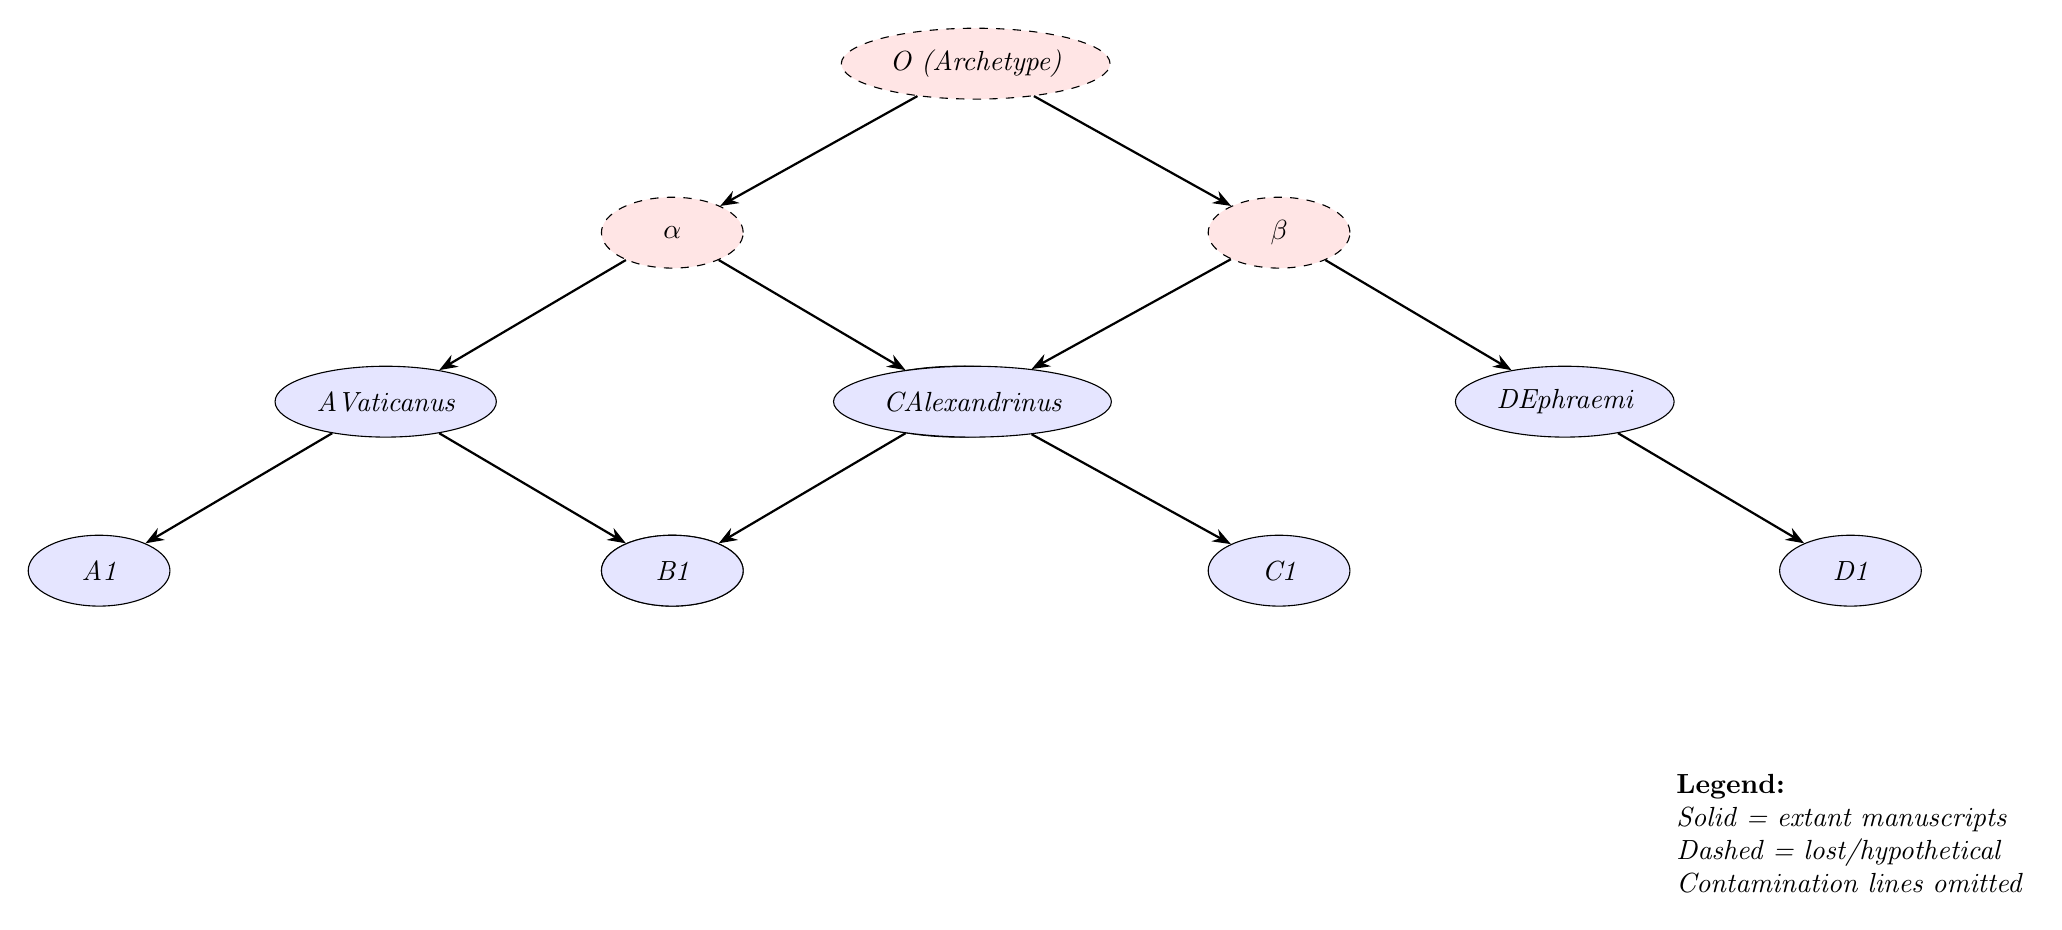
\begin{tikzpicture}[
    node distance=1.5cm and 2cm,
    ms/.style={ellipse, draw, minimum width=1.8cm, minimum height=0.9cm, fill=blue!10, font=\itshape},
    lost/.style={ellipse, draw, dashed, minimum width=1.8cm, minimum height=0.9cm, fill=red!10, font=\itshape},
    arrow/.style={-Stealth, thick},
    label/.style={font=\small, sloped, above}
]
% Archetype
\node[lost] (O) {O (Archetype)};

% First generation
\node[lost, below left=of O] (alpha) {$\alpha$};
\node[lost, below right=of O] (beta) {$\beta$};

% Second generation
\node[ms, below left=of alpha] (A) {A\\Vaticanus};
\node[ms, below right=of alpha] (B) {B\\Sinaiticus};
\node[ms, below left=of beta] (C) {C\\Alexandrinus};
\node[ms, below right=of beta] (D) {D\\Ephraemi};

% Third generation
\node[ms, below left=of A] (A1) {A1};
\node[ms, below right=of A] (A2) {A2};
\node[ms, below left=of B] (B1) {B1};
\node[ms, below right=of C] (C1) {C1};
\node[ms, below right=of D] (D1) {D1};

\draw[arrow] (O) -- (alpha);
\draw[arrow] (O) -- (beta);
\draw[arrow] (alpha) -- (A);
\draw[arrow] (alpha) -- (B);
\draw[arrow] (beta) -- (C);
\draw[arrow] (beta) -- (D);
\draw[arrow] (A) -- (A1);
\draw[arrow] (A) -- (A2);
\draw[arrow] (B) -- (B1);
\draw[arrow] (C) -- (C1);
\draw[arrow] (D) -- (D1);

% Legend
\node[below=2cm of D1, anchor=north, align=left] {
\textbf{Legend:}\\
\itshape Solid = extant manuscripts\\
\itshape Dashed = lost/hypothetical\\
\textit{Contamination lines omitted}
};
\end{tikzpicture}
\caption{Stemma codicum for a textual tradition}\label{fig:stemma}
\end{figure}

% ============================================================
% 5. Parallel Text Alignment
% ============================================================
\section{Parallel Text Alignment Visualization}
\label{sec:parallel}

\begin{figure}[htbp]
\centering
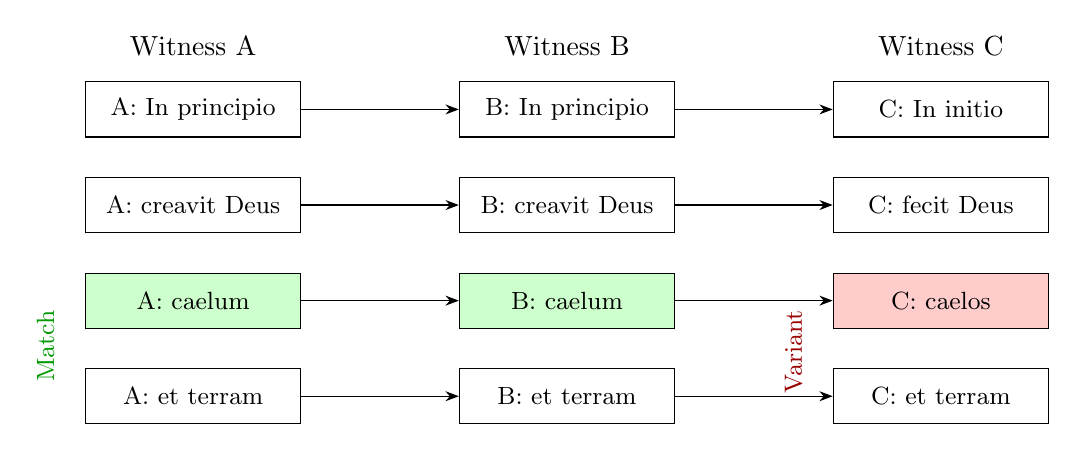
\begin{tikzpicture}[
    node distance=0.5cm,
    block/.style={rectangle, draw, minimum height=0.7cm, text width=2.5cm, align=center, font=\small},
    match/.style={rectangle, draw, fill=green!20, minimum height=0.7cm, text width=2.5cm, align=center, font=\small},
    diff/.style={rectangle, draw, fill=red!20, minimum height=0.7cm, text width=2.5cm, align=center, font=\small},
    arrow/.style={-Stealth, thin}
]
% Witness A column
\node[block] (A1) {A: In principio};
\node[block, below=of A1] (A2) {A: creavit Deus};
\node[match, below=of A2] (A3) {A: caelum};
\node[block, below=of A3] (A4) {A: et terram};

% Witness B column
\node[block, right=2cm of A1] (B1) {B: In principio};
\node[block, below=of B1] (B2) {B: creavit Deus};
\node[match, below=of B2] (B3) {B: caelum};
\node[block, below=of B3] (B4) {B: et terram};

% Witness C column
\node[block, right=2cm of B1] (C1) {C: In initio};
\node[block, below=of C1] (C2) {C: fecit Deus};
\node[diff, below=of C2] (C3) {C: caelos};
\node[block, below=of C3] (C4) {C: et terram};

% Arrows showing alignment
\draw[arrow] (A1) -- (B1);
\draw[arrow] (B1) -- (C1);
\draw[arrow] (A2) -- (B2);
\draw[arrow] (B2) -- (C2);
\draw[arrow] (A3) -- (B3);
\draw[arrow] (B3) -- (C3);
\draw[arrow] (A4) -- (B4);
\draw[arrow] (B4) -- (C4);

% Labels
\node[above=0.2cm of A1] {Witness A};
\node[above=0.2cm of B1] {Witness B};
\node[above=0.2cm of C1] {Witness C};
\node[left=0.5cm of A3, rotate=90, font=\small, green!60!black] {Match};
\node[left=0.5cm of C3, rotate=90, font=\small, red!60!black] {Variant};
\end{tikzpicture}
\caption{Parallel text alignment across three witnesses}\label{fig:parallel}
\end{figure}

% ============================================================
% 6. Coordinate Systems (Graphics)
% ============================================================
\section{3D Coordinate Systems}
\label{sec:coordsys}

\begin{figure}[htbp]
\centering
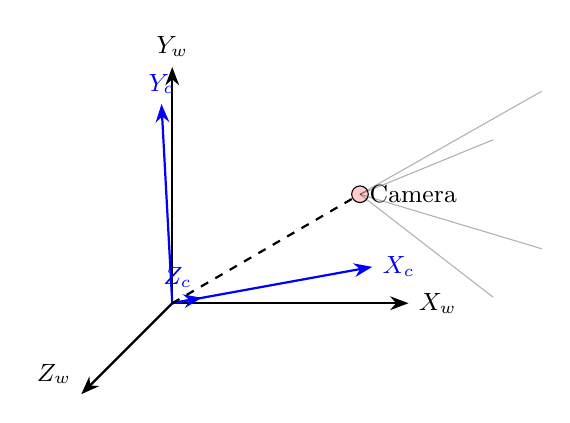
\begin{tikzpicture}[
    scale=2,
    >=Stealth,
    axis/.style={-Stealth, thick},
    vector/.style={-Stealth, thick, blue},
    label/.style={font=\small}
]
% World coordinates
\draw[axis] (0,0,0) -- (1.5,0,0) node[right, label] {$X_w$};
\draw[axis] (0,0,0) -- (0,1.5,0) node[above, label] {$Y_w$};
\draw[axis] (0,0,0) -- (0,0,1.5) node[above left, label] {$Z_w$};

% Camera coordinates (rotated)
\begin{scope}[rotate around y=30, rotate around x=-20]
\draw[vector] (0,0,0) -- (1.2,0,0) node[right, label] {$X_c$};
\draw[vector] (0,0,0) -- (0,1.2,0) node[above, label] {$Y_c$};
\draw[vector] (0,0,0) -- (0,0,1.2) node[above left, label] {$Z_c$};
\end{scope}

% Camera position
\draw[dashed, thick] (0,0,0) -- (1.5,1,0.8);
\node[fill=red!20, draw, circle, minimum size=6pt, inner sep=0] at (1.5,1,0.8) {};
\node[right, label] at (1.5,1,0.8) {Camera};

% View frustum
\draw[thin, opacity=0.3] (1.5,1,0.8) -- (2.5,1.5,1.2);
\draw[thin, opacity=0.3] (1.5,1,0.8) -- (2.5,0.5,1.2);
\draw[thin, opacity=0.3] (1.5,1,0.8) -- (2.5,1.5,0.4);
\draw[thin, opacity=0.3] (1.5,1,0.8) -- (2.5,0.5,0.4);
\end{tikzpicture}
\caption{World and camera coordinate systems with view frustum}\label{fig:coordsys}
\end{figure}

% ============================================================
% 7. BRDF Lobe Visualization
% ============================================================
\section{BRDF Lobe (Polar Plot)}
\label{sec:brdf}

\begin{figure}[htbp]
\centering
\begin{tikzpicture}
\begin{polaraxis}[
    width=8cm,
    height=8cm,
    axis lines=none,
    xtick={0,45,...,315},
    ytick=\empty,
    ymax=1,
    domain=0:360,
    samples=200
]
% Lambertian (cosine)
\addplot[fill=blue!30, draw=blue, thick, domain=0:180] ({x}, {cos(x)});
% Specular lobe (Phong-like)
\addplot[fill=red!30, draw=red, thick, domain=-30:30] ({x}, {cos(x)^10});
% GGX-like
\addplot[fill=green!30, draw=green!60!black, thick, domain=-60:60] ({x}, {1/(1+tan(x/2)^2)});
\end{polaraxis}
\node[font=\small, align=center] at (0,-4.5) {
\textbf{BRDF Lobes:}\\
Blue: Lambertian (diffuse)\\
Red: Phong (specular, n=10)\\
Green: GGX ($\alpha=0.3$)
};
\end{tikzpicture}
\caption{BRDF lobe shapes in polar coordinates}\label{fig:brdf}
\end{figure}

% ============================================================
% 8. Performance Plot (PGFPlots)
% ============================================================
\section{Performance Comparison Plot}
\label{sec:perfplot}

\begin{figure}[htbp]
\centering
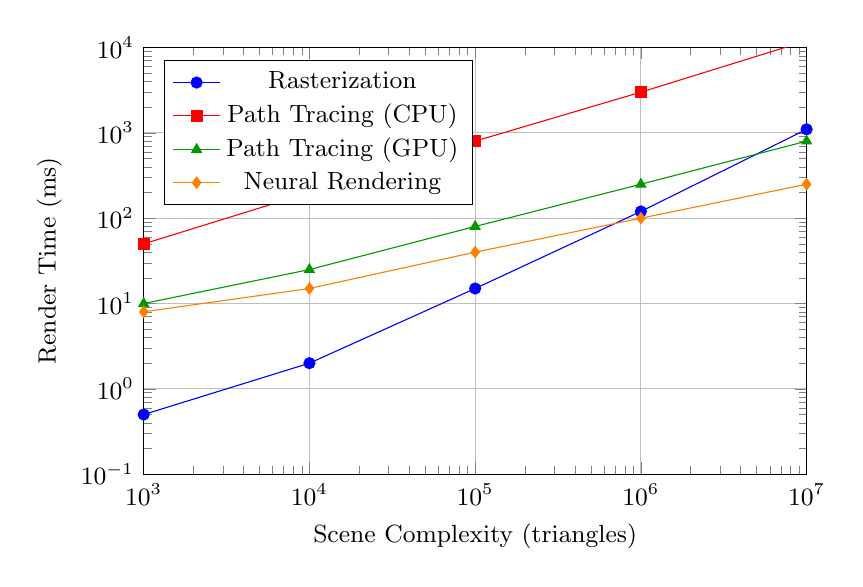
\begin{tikzpicture}
\begin{loglogaxis}[
    width=10cm,
    height=7cm,
    xlabel={Scene Complexity (triangles)},
    ylabel={Render Time (ms)},
    legend pos=north west,
    grid=major,
    xmin=1e3, xmax=1e7,
    ymin=0.1, ymax=1e4,
    tick label style={font=\small},
    label style={font=\small},
    legend style={font=\small}
]
\addplot[mark=*, blue] coordinates {
    (1e3, 0.5) (1e4, 2) (1e5, 15) (1e6, 120) (1e7, 1100)
};
\addlegendentry{Rasterization}

\addplot[mark=square*, red] coordinates {
    (1e3, 50) (1e4, 200) (1e5, 800) (1e6, 3000) (1e7, 12000)
};
\addlegendentry{Path Tracing (CPU)}

\addplot[mark=triangle*, green!60!black] coordinates {
    (1e3, 10) (1e4, 25) (1e5, 80) (1e6, 250) (1e7, 800)
};
\addlegendentry{Path Tracing (GPU)}

\addplot[mark=diamond*, orange] coordinates {
    (1e3, 8) (1e4, 15) (1e5, 40) (1e6, 100) (1e7, 250)
};
\addlegendentry{Neural Rendering}
\end{loglogaxis}
\end{tikzpicture}
\caption{Render time scaling with scene complexity}\label{fig:perf}
\end{figure}

% ============================================================
% 9. Convergence Plot
% ============================================================
\section{Monte Carlo Convergence}
\label{sec:convergence}

\begin{figure}[htbp]
\centering
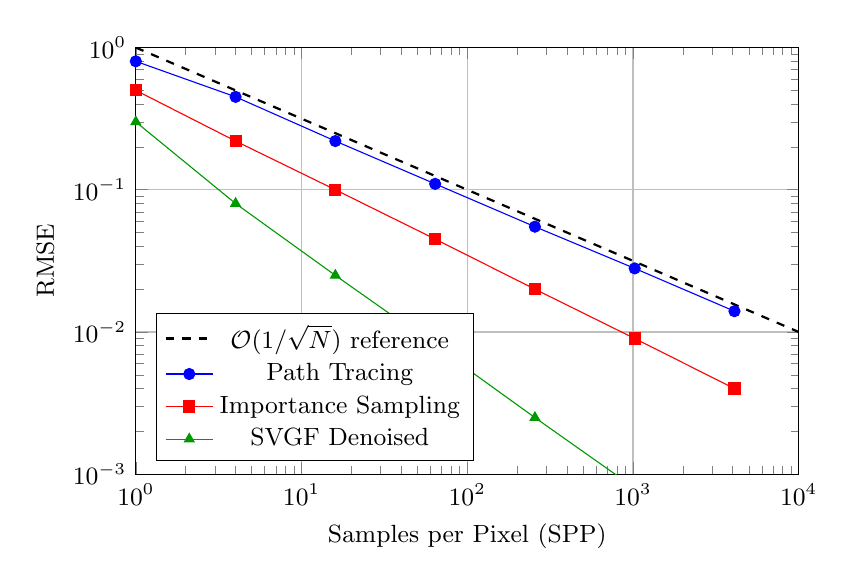
\begin{tikzpicture}
\begin{loglogaxis}[
    width=10cm,
    height=7cm,
    xlabel={Samples per Pixel (SPP)},
    ylabel={RMSE},
    legend pos=south west,
    grid=major,
    xmin=1, xmax=1e4,
    ymin=1e-3, ymax=1,
    tick label style={font=\small},
    label style={font=\small},
    legend style={font=\small}
]
% Reference 1/sqrt(N)
\addplot[dashed, black, thick] coordinates {
    (1, 1) (1e4, 1e-2)
};
\addlegendentry{$\mathcal{O}(1/\sqrt{N})$ reference}

% Path tracing
\addplot[mark=*, blue] coordinates {
    (1, 0.8) (4, 0.45) (16, 0.22) (64, 0.11) (256, 0.055) (1024, 0.028) (4096, 0.014)
};
\addlegendentry{Path Tracing}

% Importance sampling
\addplot[mark=square*, red] coordinates {
    (1, 0.5) (4, 0.22) (16, 0.1) (64, 0.045) (256, 0.02) (1024, 0.009) (4096, 0.004)
};
\addlegendentry{Importance Sampling}

% Denoised
\addplot[mark=triangle*, green!60!black] coordinates {
    (1, 0.3) (4, 0.08) (16, 0.025) (64, 0.008) (256, 0.0025) (1024, 0.0008)
};
\addlegendentry{SVGF Denoised}
\end{loglogaxis}
\end{tikzpicture}
\caption{Monte Carlo convergence rates}\label{fig:convergence}
\end{figure}

% ============================================================
% 10. Data Flow Diagram
% ============================================================
\section{Data Flow / Pipeline Stages}
\label{sec:dataflow}

\begin{figure}[htbp]
\centering
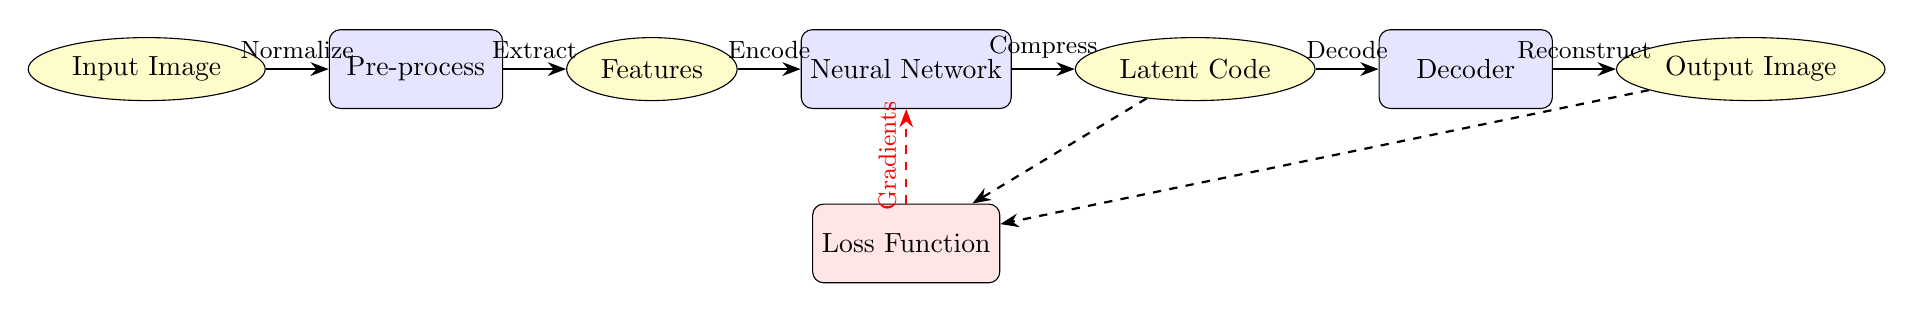
\begin{tikzpicture}[
    node distance=1.2cm and 0.8cm,
    proc/.style={rectangle, draw, rounded corners, minimum height=1cm, minimum width=2.2cm, fill=blue!10},
    data/.style={ellipse, draw, minimum height=0.8cm, minimum width=2cm, fill=yellow!20},
    arrow/.style={-Stealth, thick},
    label/.style={font=\small, above, sloped}
]
\node[data] (input) {Input Image};
\node[proc, right=of input] (pre) {Pre-process};
\node[data, right=of pre] (feat) {Features};
\node[proc, right=of feat] (net) {Neural Network};
\node[data, right=of net] (latent) {Latent Code};
\node[proc, right=of latent] (dec) {Decoder};
\node[data, right=of dec] (output) {Output Image};

\draw[arrow] (input) -- node[label] {Normalize} (pre);
\draw[arrow] (pre) -- node[label] {Extract} (feat);
\draw[arrow] (feat) -- node[label] {Encode} (net);
\draw[arrow] (net) -- node[label] {Compress} (latent);
\draw[arrow] (latent) -- node[label] {Decode} (dec);
\draw[arrow] (dec) -- node[label] {Reconstruct} (output);

% Loss
\node[proc, below=of net, fill=red!10] (loss) {Loss Function};
\draw[arrow, dashed] (latent) -- (loss);
\draw[arrow, dashed] (output) -- (loss);
\draw[arrow, dashed, red] (loss) -- node[left, label] {Gradients} (net);
\end{tikzpicture}
\caption{Neural rendering data flow with training loop}\label{fig:dataflow}
\end{figure}

% ============================================================
% 11. Manuscript Page Layout (DH)
% ============================================================
\section{Manuscript Page Layout}
\label{sec:mslayout}

\begin{figure}[htbp]
\centering
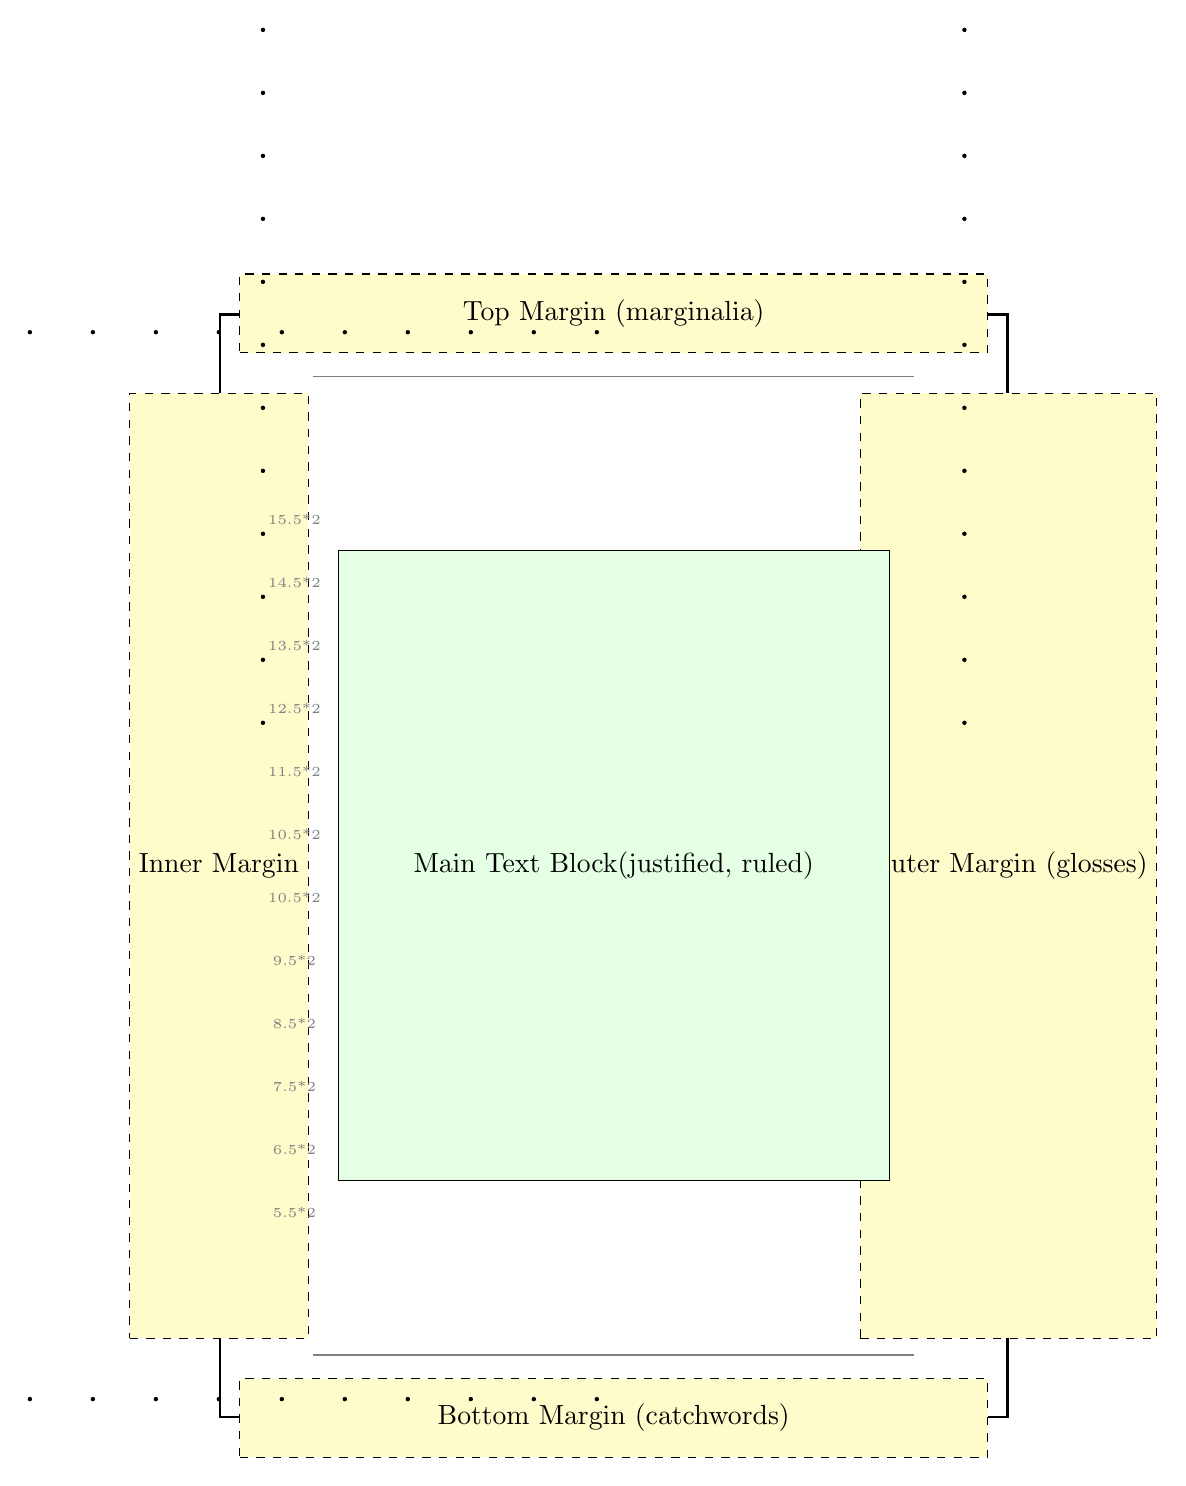
\begin{tikzpicture}[
    scale=0.8,
    page/.style={rectangle, draw, thick, minimum width=10cm, minimum height=14cm},
    block/.style={rectangle, draw, fill=blue!10, minimum height=1cm},
    margin/.style={rectangle, draw, dashed, fill=yellow!20, minimum height=0.6cm},
    textblock/.style={rectangle, draw, fill=green!10, minimum height=8cm, minimum width=7cm}
]
% Page outline
\node[page] (page) {};

% Margins
\node[margin, minimum width=9.5cm, minimum height=1cm] at (page.north) {Top Margin (marginalia)};
\node[margin, minimum width=9.5cm, minimum height=1cm] at (page.south) {Bottom Margin (catchwords)};
\node[margin, minimum width=1.5cm, minimum height=12cm] at (page.west) {Inner Margin};
\node[margin, minimum width=1.5cm, minimum height=12cm] at (page.east) {Outer Margin (glosses)};

% Text block
\node[textblock] at (page.center) {Main Text Block\\ (justified, ruled)};

% Ruling
\draw[thin, gray] ($(page.north west)+(1.5, -1)$) -- ($(page.north east)+(-1.5, -1)$);
\draw[thin, gray] ($(page.south west)+(1.5, 1)$) -- ($(page.south east)+(-1.5, 1)$);

% Line numbers
\foreach \y in {-5.5,-4.5,...,5.5} {
    \node[font=\tiny, gray] at ($(page.west)+(1.2, \y)$) {\the\numexpr 10+\y*2\relax};
}

% Pricking holes
\foreach \x in {-4.5,-3.5,...,4.5} {
    \fill[black] ($(page.north west)+(1.5+\x, -0.3)$) circle (1pt);
    \fill[black] ($(page.south west)+(1.5+\x, 0.3)$) circle (1pt);
}
\foreach \y in {-5.5,-4.5,...,5.5} {
    \fill[black] ($(page.north west)+(0.7, -1+\y)$) circle (1pt);
    \fill[black] ($(page.north east)+(-0.7, -1+\y)$) circle (1pt);
}
\end{tikzpicture}
\caption{Medieval manuscript page layout with ruling and pricking}\label{fig:mslayout}
\end{figure}

% ============================================================
% 12. Externalizing TikZ (for large documents)
% ============================================================
\section{Externalizing TikZ Figures}
\label{sec:externalize}

For large documents with many TikZ figures, use externalization
to compile figures separately and include as PDFs:

\begin{verbatim}
% In preamble:
\usetikzlibrary{external}
\tikzexternalize[prefix=figures/]

% Compile with: pdflatex -shell-escape document.tex
% Or in Overleaf: enable "Shell Escape" in settings
\end{verbatim}

Each figure is compiled once and cached. Subsequent runs
are much faster.

% ============================================================
% 13. Color Definitions for Consistency
% ============================================================
\section{Color Palette Definitions}
\label{sec:colors}

\begin{figure}[htbp]
\centering
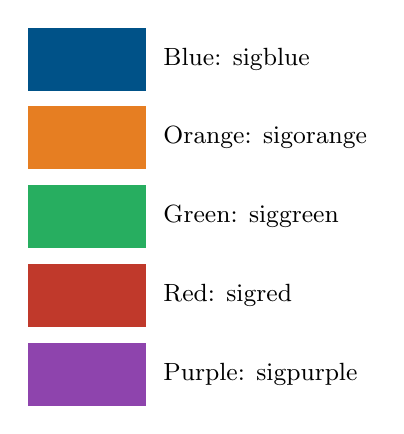
\begin{tikzpicture}
% Define palette
\definecolor{sigblue}{RGB}{0, 82, 136}
\definecolor{sigorange}{RGB}{230, 126, 34}
\definecolor{siggreen}{RGB}{39, 174, 96}
\definecolor{sigred}{RGB}{192, 57, 43}
\definecolor{sigpurple}{RGB}{142, 68, 173}

\foreach \c/\n/\i in {
    sigblue/Blue/0,
    sigorange/Orange/1,
    siggreen/Green/2,
    sigred/Red/3,
    sigpurple/Purple/4
} {
    \fill[\c] (0,-\i) rectangle (1.5,-\i+0.8);
    \node[right, font=\small] at (1.6,-\i+0.4) {\n: \c};
}
\end{tikzpicture}
\caption{Consistent color palette for paper figures}\label{fig:colors}
\end{figure}

\end{document}